\documentclass[notes, xcolor=dvipsnames]{beamer}    

\usetheme{Berkeley}

\setbeamertemplate{footline}[frame number]

\usepackage{amsmath}
\usepackage{inputenc}
\usepackage{graphicx}
\usepackage{hyperref}

%Title too big, perhaps we can shorten it somehow ?
\title{Constraint based scheduling of Weakly Consistent C programs for Reconfigurable Hardware}
\author{Akshay Gopalakrishnan}

\begin{document}
    
    \begin{frame}

        \maketitle

    \end{frame}

    \section{Introduction}
    \begin{frame}{Recap: HLS Design Flow}

        \begin{figure}
            \makebox[\textwidth][c]{
                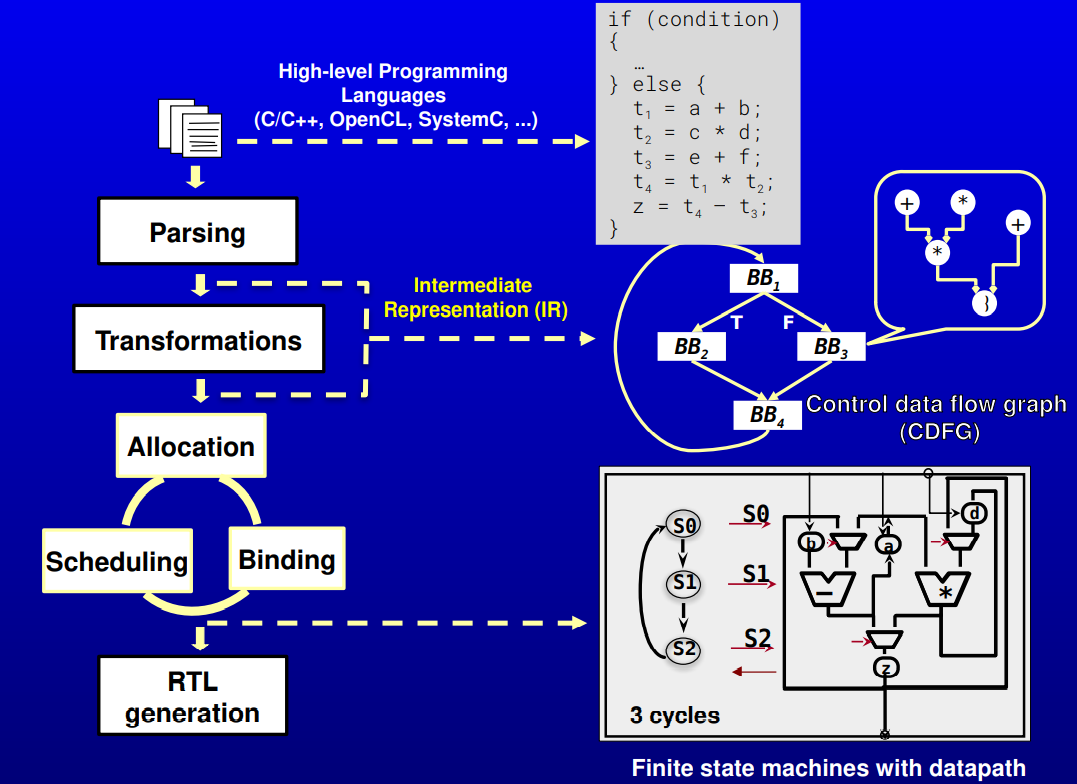
\includegraphics[scale=0.4]{HLS-flow.PNG}
            }
        \end{figure}

        Focus on the scheduling and transformation phases.
        
    \end{frame}

    \section{Concurrent Program Synthesis}
    \begin{frame}{Mapping Threads to Reconfigurable Hardware}

        \begin{figure}
            \makebox[\textwidth][c]{
                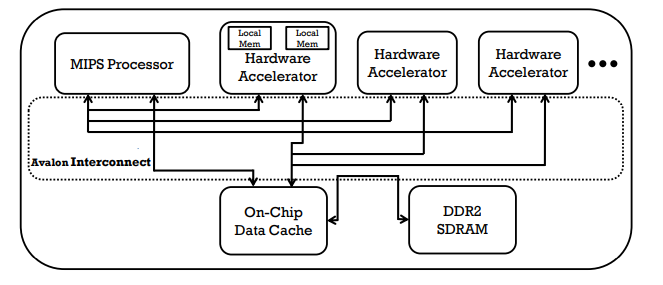
\includegraphics[scale=0.7]{Pthread-to-FPGA.PNG}
            }
        \end{figure}

        Each thread mapped to a unique hardware accelerator. 

    \end{frame}

    \begin{frame}{Concrete Example: Producer Consumer System}

        \begin{figure}
            \makebox[\textwidth][c]{
                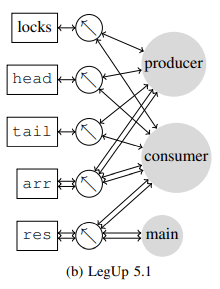
\includegraphics[scale=0.7]{ProdCons-FPGA.PNG}
            }
        \end{figure}

        Assumption is we have infinite supply of accelerators

    \end{frame}

    \section{Limitation from Previous Work}
    \begin{frame}{Resource Constraint: Limited Hardware Accelerator}


        \begin{figure}
            \makebox[\textwidth][c]{
                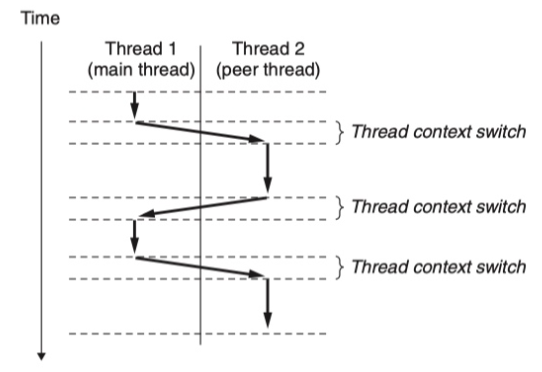
\includegraphics[scale=0.7]{ContextSwitchThreads.PNG}
            }
        \end{figure}

        Schedule involves additional context switch cycles.
        
    \end{frame}

    \section{Proposed Remedy}
    \begin{frame}{Proposed Solution}

        Perform inlining at the transformation phase. 

        Saves context switch clock cycles.
        
    \end{frame}

    \begin{frame}{Advantage in Weak Memory Setting}

        \begin{columns}
            
            \begin{column}{0.5\textwidth}

                \begin{figure}
                    \makebox[\textwidth][c]{
                        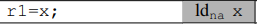
\includegraphics[scale=0.7]{t1-na-ld.PNG}
                    }
                \end{figure}
                                
            \end{column}

            \begin{column}{0.5\textwidth}

                \begin{figure}
                    \makebox[\textwidth][c]{
                        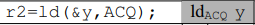
\includegraphics[scale=0.7]{t2-acq-ld.PNG}
                    }
                \end{figure}
                        
            \end{column}

        \end{columns} 

        \begin{figure}
            \makebox[\textwidth][c]{
                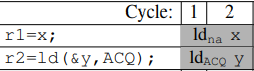
\includegraphics[scale=0.7]{t1-t2-inline.PNG}
            }
        \end{figure}

        2 clock cycles only ! 
        
    \end{frame}

    \begin{frame}{Methodology}

        \begin{itemize}
            \item Insert AST node for threads in assignment code base. 
            \item Programs assumed to be given in the form of memory accesses ONLY.
            \item Encode dependencies for weak atomics from previous work.
            \item Add thread inlining transformation.
            \item Add analysis pre-inlining to identify which threads to inline. 
            \item Compare schedules.
        \end{itemize}

        Testbench will be mainly custom-made examples in addition to Message Passing and Producer Consumer algorithms from previous work.

    \end{frame}
    
    \section{Thank you!}
    \begin{frame}{Thank you!}

        Some paper references.
        \begin{itemize}
            \item \href{https://janders.eecg.utoronto.ca/pdfs/james.pdf}{Pthreads to Hardware}
            \item \href{https://johnwickerson.github.io/papers/feetup_TC.pdf}{Relaxed Memory C Programs to Hardware}
            \item \href{https://johnwickerson.github.io/papers/cats_TVLSI.pdf}{Global Analysis for Efficient Scheduling of Concurrent C programs for Hardware}
            \item \href{http://www.cs.kent.edu/~walker/papers/dtsched.pdf}{Scheduling Problem}
        \end{itemize}

        Any feedback? 

        
    \end{frame}

\end{document}